\documentclass[tikz,border=6pt]{standalone}
\usepackage{amsmath,amssymb}
\usepackage{lmodern}
\usepackage[T1]{fontenc}
\usetikzlibrary{decorations.pathreplacing}
\definecolor{normalgreen}{RGB}{19,130,81}
\definecolor{subblue}{RGB}{40,105,181}
\definecolor{thresholdyellow}{RGB}{200,151,20}
\definecolor{inforange}{RGB}{221,112,41}
\definecolor{nanred}{RGB}{188,55,70}
\begin{document}
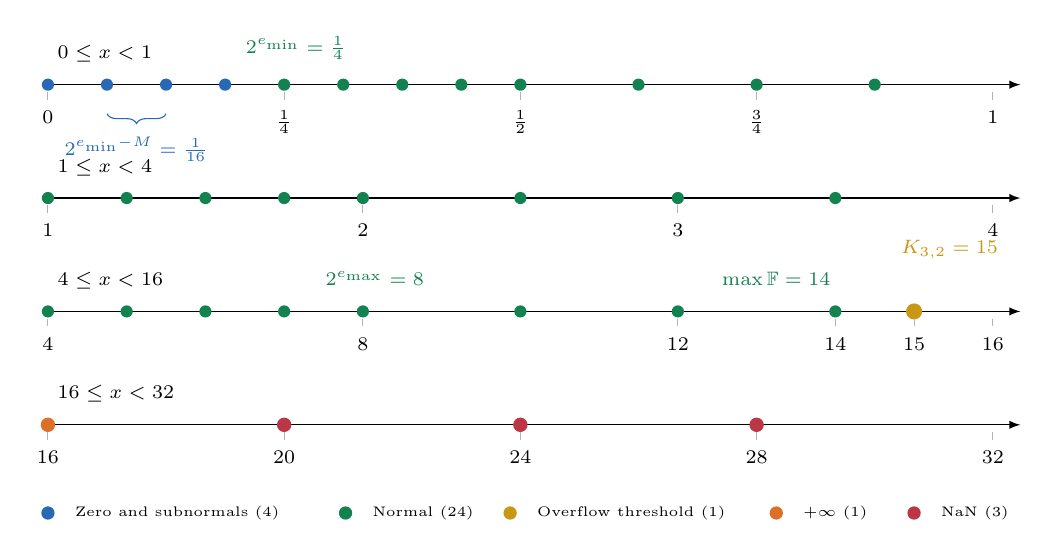
\begin{tikzpicture}[x=1cm,y=1cm,>=latex,every node/.style={font=\footnotesize}]
% Each strip is locally linear; the final strip represents encoding slots.
\foreach \yy/\region in {5.0/{$0\le x<1$},3.56/{$1\le x<4$},2.12/{$4\le x<16$},0.68/{$16\le x<32$}}{
  \draw[thin,->] (0,\yy) -- (12.35,\yy);
  \node[anchor=south west,font=\scriptsize] at (0,\yy+.16) {\region};
}
\foreach \v in {0,0.0625,0.125,0.1875} {\fill[subblue] ({12*\v},5.0) circle (2.2pt);}
\foreach \v in {0.25,0.3125,0.375,0.4375,0.5,0.625,0.75,0.875} {\fill[normalgreen] ({12*\v},5.0) circle (2.2pt);}
\foreach \v in {1,1.25,1.5,1.75,2,2.5,3,3.5} {\fill[normalgreen] ({4*(\v-1)},3.56) circle (2.2pt);}
\foreach \v in {4,5,6,7,8,10,12,14} {\fill[normalgreen] ({(\v-4)},2.12) circle (2.2pt);}
% Overflow threshold is NOT a floating-point value: point only, no vertical line.
\fill[thresholdyellow] (11,2.12) circle (2.9pt);
% Sparse axes and mathematical landmarks.
\foreach \x/\t in {0/$0$,3/$\frac14$,6/$\frac12$,9/$\frac34$,12/$1$}{
 \draw[gray!60] (\x,4.91)--(\x,4.81);
 \node[anchor=north,font=\scriptsize] at (\x,4.79){\t};}
\foreach \x/\t in {0/$1$,4/$2$,8/$3$,12/$4$}{
 \draw[gray!60] (\x,3.47)--(\x,3.37);
 \node[anchor=north,font=\scriptsize] at (\x,3.35){\t};}
\foreach \x/\t in {0/$4$,4/$8$,8/$12$,10/$14$,11/$15$,12/$16$}{
 \draw[gray!60] (\x,2.03)--(\x,1.93);
 \node[anchor=north,font=\scriptsize] at (\x,1.91){\t};}
\node[anchor=south,font=\scriptsize,text=normalgreen] at (3.15,5.19){$2^{e_{\min}}=\frac14$};
\node[anchor=south,font=\scriptsize,text=normalgreen] at (4.15,2.32){$2^{e_{\max}}=8$};
\node[anchor=south,font=\scriptsize,text=normalgreen] at (9.25,2.32){$\max\mathbb{F}=14$};
\node[anchor=south,font=\scriptsize,text=thresholdyellow] at (11.45,2.66){$K_{3,2}=15$};
% One brace for the minimum subnormal spacing: from 1/16 to 1/8.
\draw[decorate,decoration={brace,amplitude=3.5pt,mirror},subblue,thin]
 (0.75,4.63)--(1.50,4.63)
 node[midway,below=5pt,font=\scriptsize,text=subblue] {$2^{e_{\min}-M}=\frac1{16}$};
% Special encoding slots, NOT real values 16, 20, 24, 28.
\fill[inforange] (0,0.68) circle (2.6pt);
\foreach \x in {3,6,9}{\fill[nanred] (\x,0.68) circle (2.6pt);}
\foreach \x/\t in {0/$16$,3/$20$,6/$24$,9/$28$,12/$32$}{
 \draw[gray!60] (\x,0.59)--(\x,0.49);
 \node[anchor=north,font=\scriptsize] at (\x,0.47){\t};}
% Single five-category legend beneath all four strips.
\fill[subblue] (0,-0.44) circle (2.4pt);
\node[anchor=west,font=\tiny] at (.22,-0.44){Zero and subnormals (4)};
\fill[normalgreen] (3.78,-0.44) circle (2.4pt);
\node[anchor=west,font=\tiny] at (4.00,-0.44){Normal (24)};
\fill[thresholdyellow] (5.87,-0.44) circle (2.4pt);
\node[anchor=west,font=\tiny] at (6.09,-0.44){Overflow threshold (1)};
\fill[inforange] (9.25,-0.44) circle (2.4pt);
\node[anchor=west,font=\tiny] at (9.47,-0.44){$+\infty$ (1)};
\fill[nanred] (11.00,-0.44) circle (2.4pt);
\node[anchor=west,font=\tiny] at (11.22,-0.44){NaN (3)};
\end{tikzpicture}
\end{document}
